% This template was created by Ben Mitchell
% for Dr. Sheppard's AI class, CS 335/435, spring 08.

% For those who want to learn LaTeX, this is a decent place to start:
% http://en.wikibooks.org/wiki/LaTeX
% Note that the proper pronunciation is "la tek", not "lay teks".
%
% There are lots of latex tutorials and primers online; just be careful with
% google images.

\documentclass[12pt,letterpaper]{article}

\usepackage{amsmath, amsthm, graphicx, multicol, natbib}

\title{AI Learning Polar Tic-Tac-Toe: \\ Simple Hurestic, Naive Bayes, Temporal Difference Neural Network, Minimax}
\author{Jacob Barthelmeh, Kaleb Himes, Angelica Davis}

\begin{document}
\maketitle

\begin{abstract}
This is an experiment to compare the ability of four different algorithms to win a polar tic tac toe game. The four algorithms used are; a simple heuristic, Naive Bayes Network, Temporal Difference Neural Network (TDNN) and the Minimax Algorithm. Algorithms are compared in their ability to learn and their ability to win when competing against each other.
\end{abstract}

\section{Introduction}
\begin{quote}
`` 
In the first section of your paper, which should be entitled ``Introduction,''
you should introduce the subject of your paper to the reader.  There are several
components to this.  You probably want to begin by talking about what problem
your work is trying to solve, and why it is a problem worth trying to solve.
Explain to your reader why they should care.  This is also a good time to
introduce basic nomenclature related to your subject.  You can assume that your
reader is a reasonably well educated individual and has some knowledge of
computer science, but you should not assume that they are an expert in your field.  You have
spent a bunch of time studying your topic (in this case, game AI), but
your reader may not have.  Take the time to bring him or her up to speed; this
is what the introduction is all about.

The introduction in a real paper is generally several pages, but yours does not
need to be that long for this assignment.  It should, however, be long enough to
convey the information you need to convey.  It should move from the initial, high level
overview of the topic to a more detailed description of what other related work
has been done on the topic, and any other background information needed to
understand the later parts of the paper.  For example, you should talk about the nature
of game search in general, and what other work has been
done to solve this important problem.  More specific details of the algorithms and
techniques you used should wait for later sections.

Because your introduction discusses prior related work, you should be sure to
properly cite that prior related work. An example citation is included here
If your introduction does not have at
least a couple of citations, then it is either inadequate in scope, or it fails
to properly cite works referenced.  Later sections of the
paper should also contain proper citations where needed, but the bulk of the
citations in any given paper can usually be found in the introduction or a 
separate related works section, as that
is where the most related publications are discussed.
"
\end{quote}

Use of AI in industry and commercial settings is on the rise. Such as with the use of TDNN's in robots 
\cite{robotTDNN}.
 
Minimax algorithms have been used in chess and are well suited for games \cite{flyingMinimax}. We also hypothisise that the minimax algorithm will perform best when implemented to play polar tic-tac-toe.

Previous work with the TDNN has been done on the backgammon board game \cite{stanfordTDNN}. It has shown to be able to play at a grand master level in backgammon. Here it will be implemented to make decisions on moves with the polar tic-tac-toe game. In the TDNN implementations gradient descent is used to update the weight values \cite{gradientTDNN}.

This paper is divided into an explenation of the problem followed by an explenation of each algorithm implemented. After defining the problem and showing the algorithms used there is a section on the experimental methods and on the results that came from conducting the experiment. The end of the paper has sections to discuss the results of the experiment and at the very end a conclusion.


\section{Problem Statement}
Algorithms will be used to play Polar Tic-Tac-Toe. The game is played by alternating turns of who gets to pick a move on the board. Spots picked are represented visually by a O or an X indicating which player has chosen the spot. A player having 4 spots in a row, either diagonally or in a straight line, constitutes as a win. Algorithms being experimented with will attempt to learn information about the state space of the game, to make perdictions on which move to make and ultimatly try to not lose.

\subsection{Traditional Minimax Search}
The Minimax algorithm used checks at each ply for the maximize value when looking for player ones potential moves. When playing as player two it looks to minimize the possible utility value. An adjustibale parameter set for the algorithm is the depth at which it searchs. Values are assigned by finding the max or min of the next ply. A terminating node with a win condition for player one is assigned the value of 5 and a loss condition is assigned -5. For ties the value of 0 is assigned to the node. All nodes in the tree are initialized with the value returned from the simple heuristic if player one, if player two than the node value is initialized as 0. 

\subsection{Minimax with Alpha-Beta Pruning}
 The ability to use Alpha-Beta Pruning is something that can be adjusted at runtime. It uses almost the same algorithm as the regualer Minimax but has the added check of alpha and beta values. Alpha is set to negative infinity and beta is set to positive infinity when the alpha-beta algorithm is started. This is to insure that an alpha and beta value will be found and that node values will not be over looked while the algorithm is operating. When looking for a minimum value for the next move if the value found is less than alpha the node is returned and the rest of the nodes are not explored. If the value is not less than or equal to alpha than beta is set to the minumum between the current beta value and the current node being explored. When looking for a maximum value for the next move if the value found for the current node being explored is less than or equal to the current beta value than the current node is returned and the rest of the nodes in that ply are not explored. If the value is less than the current beta value than the alpha value is updated to be the maximum value of either the current alpha value or the current node value. 

In our implementation the Alpha-Beta Pruning can be called on an exisiting stored Minimax tree. This works by starting at the head of the tree and recursivily finding the max value or min value from possible moves while keeping track of an alpha value and beta value.  It then marks nodes that the Alpha-Beta Pruning algorithm decided not to visit so that they will not be explored in the future either. 


\subsection{Heuristic Functions}

In the simple heuristic implementation, the heuristic value is the number of similar player pieces in a line adjacent to each other that include the play to be evaluated. This value ranges from one to three since a value of four signifies a win. This can be exploited to make a move by determining from all possible moves which has the highest heuristic value. This heuristic is admissible but not the closest to the actual heuristic it could be since there is a condition where there could be two in a row with a space than a another spot where the player had moved. In this case the actual heuristic value should be three but will be evaluated to two.

\[
V^\pi(s)=\max_{a in \mathcal{A}} \left[ R(s,a) + \gamma \sum_{s' \in \mathcal{S}} P(s'|s,a) V(s') \right].
\]

\begin{figure}
\begin{center}
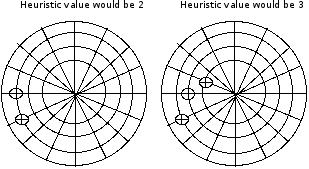
\includegraphics[width=4in]{heu.png}
\end{center}
\caption{Simple Heuristic Examples}
\label{heuristicExample}
\end{figure}

\subsection{Win Checking with Resolution}
In this section, you will describe your win checker and how you specified your rules. 
You should include the rules if there are not too many of them. Otherwise, list the most important
ones (but be sure to include all of the rules in your design document). You also need to describe 
your unification procedure and your resolution procedure. This is not the place to include code; 
however, you may provide pseudocode if you think it will help the description.

\subsection{Game Evaluation with Classifiers}
Classifing the board is done with a Naive Bayes network. 

\subsection{Temproal Diffrence Neural Network}
When training the TDNN the first 20 games are trained against a random player. This is in hopes of rudecing the risk of falling into an early local minumum. The remander of n games chosen to be trained by a user is than done by pitting the current TDNN against itself. After each game is played the final result is evaluated and each state leading up to the result is compared to the perdiction given by the network. Gradient descent is than done using the error of the network and allowing for adjustments to be made to the networks weights. The following equation is used to adjust weights in the network. 
\[
{\triangle} w_t = \alpha (V _{t + 1} - V _t)  \overset{t}{\sum_{k = 1}} {\gamme}^{t - k} {\nabla}_w V_k
\]
Where alpha is the learning rate and V is the perdicted output.

For each game the network is trained for both players, having the weights adjusted from both players perspectives after each game has ended.

The topology of the network is 48 inputs, one hidden layer with 40 nodes, and 3 output nodes. 48 input nodes to represent each possible state for a move and 3 output nodes; one for player 1 win, one for player 2 win, and one for a tie perdicted. 

\section{Experimental Methods}
\begin{quote}
`` 
In this section, you describe your experimental methodology; this is where you talk
about your data and what you did with it.  Talk about what sorts of experiments
you performed, and how you validated them.  For example, if you used self-play
or you experimented with a human playing with the computer, you would say that 
you used it, define what it is, and discuss how you implemented it.  

Since this project includes several requirements to be satisfied, this is where you describe
how those requirements are tested, and how the resulting features are being compared.
A well constructed experiment (and your description of that experiment) will go a long
way towards demonstrating that you met the project's requirements.
’’
\end{quote}

In conducting experiments with the implemented algorithms we had them compete against each other in a 1000 games each. All algorithms competed against the other 3 and also against a random player. To get the performance result of using alpha beta pruning on minimax it will also compete against the other 3 algorithms and against a random player. 


\newpage

\begin{table}
\begin{center}
\begin{tabular}{|c||c|c|c|c|}
\hline
& vs & win & tie & loss\\
\hline \hline
TDNN & Minimax & 0 & 0 & 1000\\
\hline 
TDNN & Simple Heuristic & 0 & 0 & 1000\\
\hline 
TDNN & Navie Bayes & 507 & 0 & 493\\
\hline 
TDNN & Random & 948 & 0 & 52\\
\hline 
\end{tabular}
\end{center}
\caption{Tempral Diffrence Neural Network performance with 40 hidden nodes}
\label{TDNNtable}
\end{table}

\begin{table}
\begin{center}
\begin{tabular}{|c||c|c|c|c|}
\hline
& vs & win & tie & loss\\
\hline \hline
Minimax & TDNN & 1000 & 0 & 0\\
\hline 
Minimax & Simple Heuristic & 476 & 0 & 524\\
\hline 
Minimax & Navie Bayes & 1000 & 0 & 0\\
\hline 
Minimax & Random & 979 & 1 & 20\\
\hline 
Minimax with Pruning & TDNN & 1000 & 0 & 0\\
\hline 
Minimax with Pruning & Simple Heuristic & 474 & 0 & 526\\
\hline 
Minimax with Pruning & Naive Bayes & 1000 & 0 & 0\\
\hline 
Minimax with Pruning & Random & 982 & 1 & 17\\
\hline 
\end{tabular}
\end{center}
\caption{Minimax Performance with depth of 2}
\label{MinimaxTable}
\end{table}


\begin{table}
\begin{center}
\begin{tabular}{|c||c|c|c|c|}
\hline
& vs & win & tie & loss\\
\hline \hline
Naive Bayes & TDNN & 487 & 0 & 513\\
\hline 
Naive Bayes & Simple Heuristic & 0 & 0 & 1000\\
\hline 
Naive Bayes & Minimax & 0 & 0 & 1000\\
\hline 
Naive Bayes & Random & 936 & 1 & 64\\
\hline 
\end{tabular}
\end{center}
\caption{Naive Bayes Performance}
\label{NaiveBayesTable}
\end{table}

\begin{table}
\begin{center}
\begin{tabular}{|c||c|c|c|c|}
\hline
& vs & win & tie & loss\\
\hline \hline
Simple Heuristic & TDNN & 1000 & 0 & 03\\
\hline 
Simple Heuristic & Minimax & 494 & 0 & 506\\
\hline 
Simple Heuristic & Navie Bayes & 1000 & 0 & 0\\
\hline 
Simple Heuristic & Random & 991 & 0 & 9\\
\hline 
\end{tabular}
\end{center}
\caption{Simple Heuristic Performance}
\label{HeuristicTable}
\end{table}

\begin{table}
\begin{center}
\begin{tabular}{|c||c|}
\hline
& win percentage\\
\hline \hline
TDNN & 36.4\\
\hline 
Simple Heuristic & 87.1\\
\hline 
Navie Bayes & 35.6\\
\hline 
Minimax & 86.4\\
\hline 
Minimax with Pruning & 86.4\\
\hline 
Random & 3.6\\
\hline 
\end{tabular}
\end{center}
\caption{Win percentage of algorithms in experiment}
\label{WinPercentTable}
\end{table}

\begin{figure}
\begin{center}
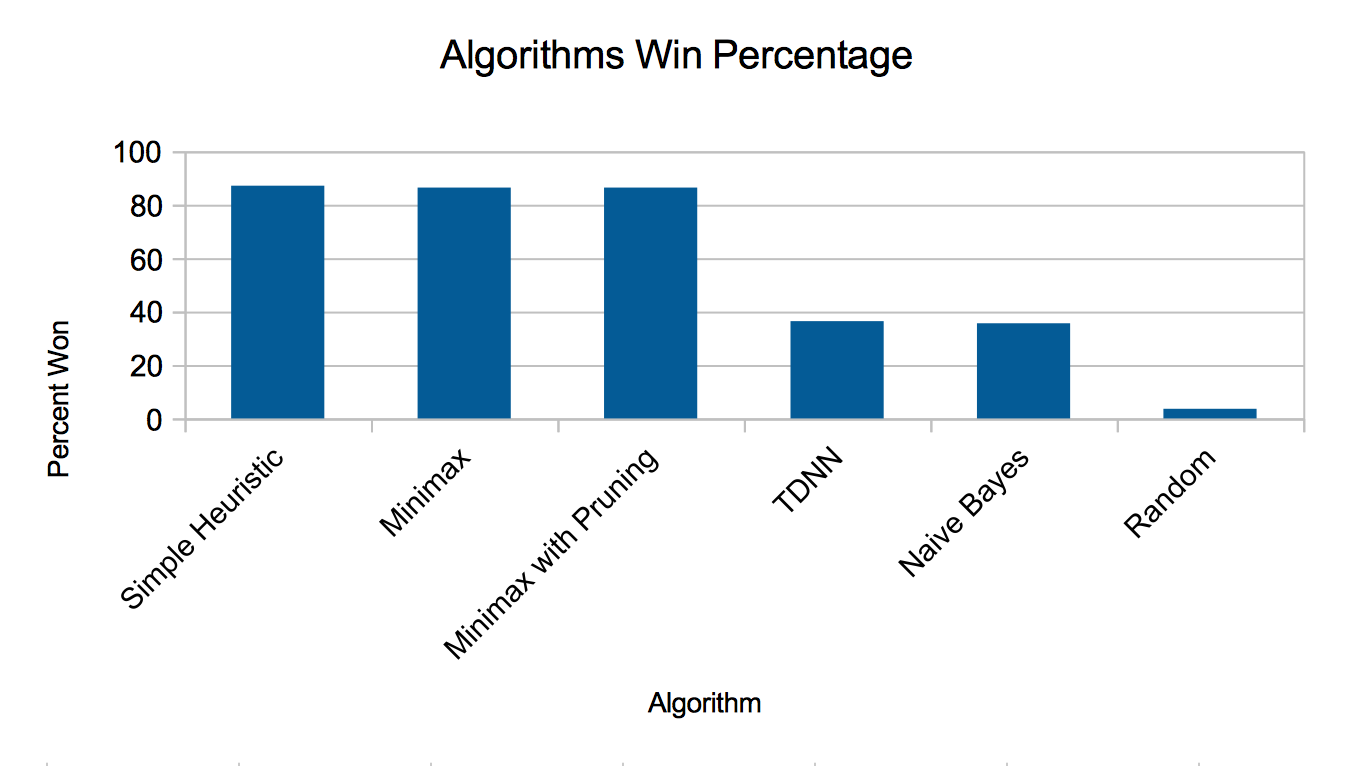
\includegraphics[width=7in]{winpercent.png}
\end{center}
\caption{Win Percentage}
\label{WinGraph}
\end{figure}

The results section should contain your results.  It should \emph{not} contain
your interpretation of those results.  That comes later.  This section should be
made up primarily of graphs and tables that show your data.  You should also
have a small amount of text describing what each of the tables and graphs shows,
since the caption on the figures should be short.  Having text describing the
specifics of the experiment that led to that particular table would also be
good.  

I am not going to tell you exactly what tables or graphs you should have here,
since it will depend a bit on your results.  You should be sure that your
results section contains sufficient data to support your conclusions about the
relative strengths and weaknesses of the different algorithms.  You should also
be sure that your data is complete; that is, do not leave data out simply because
it does not support the point you are trying to make.

You should also be sure that your results are clear and interpretable.  Seven
pages of raw binary data will do nothing to edify your reader.  Similarly, a
1 inch square graph with 12 lines plotted on it will be difficult to extract
meaning from, as will a graph with poor (or no) labels on the axes.  Your
results should be legible both on screen and in hard copy. By the way, do
not rely on color difference to make your points since many people read
black-and-white print outs of the papers (including your instructor).

You do not want to present results that are just raw data, since that is hard to
interpret.  But you do not want to be overly abstract, either, since that leads to
results that have little or no meaning (e.g., ``the average over all different
data sets, algorithms, and parameters'' is a completely useless statistic for
comparing algorithms).

\section{Discussion}
The discussion section is where you discuss your interpretation of the data you
presented in the results section.  This is where you tell the reader how great
your algorithm is, and how interesting it is that \emph{this} performed better
than \emph{that} on some given data set.  You can also speculate about causes
for interesting behaviors; for example, if you think you might know why it fails
so badly on some particular case, or if you have an insight into why it did well
on another case.  You do not want to be making wild guesses, but as long as you
make it clear that you are not making claims of factual proof, you can go out on
a limb a little.  For example,

\begin{quote}
``In most cases, algorithm A outperforms algorithm B with a significance of
99.8\%.  However, as can be seen from Figure when applied to
the E. E. Smith data set, algorithm A does no better than random chance.  It
seems likely that the failure of algorithm A to learn is due to the extremely
sparse distribution of that data set.  Because of algorithm A's heavy reliance
on data being densely sampled from the true underlying distribution, any sparse
data set is likely to show this behavior.''
\end{quote}

\section{Conclusions}
The conclusion section should be relatively short, and should not be a summary
of your paper.  It should, however, bring up what you learned and what impact
your results have on the rest of the field (and society as a
whole, if applicable).  You should conclude, and bring your paper to an  end
with any parting thoughts that are appropriate.

Certain types of papers can be ended with a ``Summary'' section instead of a
``Conclusions'' section, in which case you would, in fact, summarize the main
points of your paper.  For this paper, you should write a Conclusions section,
not a Summary.

Conclusions also often contain information about what else you would like
to do.  Sometimes this is a separate subsection, or even a section, entitled
``Future Work.''  The basic idea here is to talk about what the next steps to
take would be.  This is of benefit to others who are interested in your
work and may want to help advance it.  It is also a chance for you to
acknowledge shortcomings in your work; since we never have infinite time to
prepare a paper, there are always more experiments that would have been nice to
include.  If you list them as future work, then it at least makes it clear that
you did not do those things because you didn't have time, rather than because you
didn't realize that they were important to do.

In your paper, you should include a brief discussion of avenues for possible
future work in your Conclusions section.  It should be tied in with the rest of
your conclusion, and should not be an unrelated section tacked on the end (or
the middle).

\newpage

\bibliographystyle{plain}
\bibliography{reffrences}
\nocite{*}

\end{document}
